\documentclass{article}
\usepackage[utf8]{inputenc}
\usepackage{amsmath,amsfonts,amssymb,amsthm,mathtools}
\usepackage{parskip}
\usepackage{color}
\usepackage{booktabs}
\usepackage{hyperref}
\usepackage{tikz}
\usepackage[framemethod=tikz]{mdframed}
\usepackage{float}
\usepackage{placeins}
\usepackage{subcaption}
\usepackage{graphicx}

\definecolor{blue}{RGB}{38,139,210}
\definecolor{cyan}{RGB}{42,161,152}
\definecolor{violet}{RGB}{108,113,196}
\definecolor{red}{RGB}{220,50,47}
\definecolor{base01}{RGB}{88,110,117}
\definecolor{base02}{RGB}{7,54,66}
\definecolor{base03}{RGB}{0,43,54}

\usetikzlibrary{calc,shapes,positioning}

\newtheorem{exercise}{Exercise}
\newtheorem{answer}{Answer}

\newcommand{\dd}[2][]{\frac{\partial #1}{\partial #2}}
\newcommand{\dt}[2][]{\frac{d #1}{d #2}}
\newcommand{\dL}{\dt[{\L}]}
\newcommand{\dLi}{\dt[{\Li}]}
\newcommand{\dLmb}{\dt[{\Lmb}]}
\newcommand{\dLfb}{\dt[{\Lfb}]}
\newcommand{\yh}{\hat{y}}

\newcommand{\x}{\mathbf{x}}
\newcommand{\y}{\mathbf{y}}
\newcommand{\logits}{\ell}
\newcommand{\vlogits}{\boldsymbol{\logits}}

\newcommand{\bracket}[3]{\left#1 #3 \right#2}
\newcommand{\sqb}{\bracket{[}{]}}
\newcommand{\ab}{\bracket{\langle}{\rangle}}
\renewcommand{\b}{\bracket{(}{)}}
\newcommand{\abs}{\bracket{\lvert}{\rvert}}

\newcommand{\W}{\mathbf{W}}
\newcommand{\Wkey}{\mathbf{W}_\text{k}}
\newcommand{\Wquery}{\mathbf{W}_\text{q}}
\newcommand{\A}{\mathbf{A}}
\newcommand{\B}{\mathbf{B}}
\newcommand{\X}{\mathbf{X}}
\newcommand{\Y}{\mathbf{Y}}
\renewcommand{\H}{\mathbf{H}}
\renewcommand{\a}{\mathbf{a}}
\newcommand{\h}{\mathbf{h}}
\newcommand{\p}{\mathbf{p}}




\title{EMAT31530: Large Language Models}
\author{Laurence Aitchison}
\date{}

\begin{document}

\maketitle

One of the most impressive developments in modern AI is ``Large Language Models'' (LLMs).
If you haven't already had a play with \href{https://chat.openai.com}{ChatGPT}, you really should.
It is quite amazing.

This week, we're going to look at the basic building blocks that make LLMs such as ChatGPT work.

\section{How text is represented in the computer}

Text is represented in programming as a ``string''.
For instance, if you do:
\begin{verbatim}
>>> a = "Fine tuning is fun for all!"
\end{verbatim}
That's a string.
You can do various operations on strings.  For instance, we can take the first 10 characters:
\begin{verbatim}
>>> a[:10]
"Fine tunin"
\end{verbatim}
See notebooks for more details.

\section{Tokenisation}

Neural networks work with numbers, not text/strings.
So first question is: how do we convert text/strings to numbers (and back).
The answer is ``tokenization''.

In tokenization, we associate substrings (usually but not always words) such as `` is'' with an integer index.
As an example:
\begin{center}
  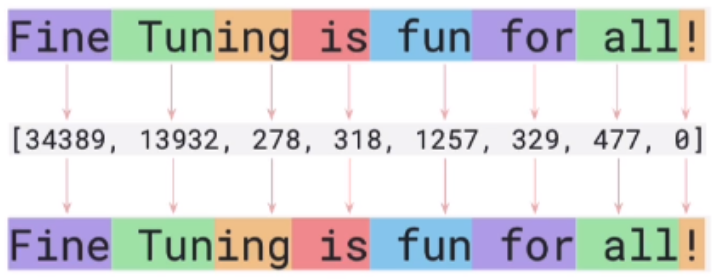
\includegraphics[width=0.6\textwidth]{token_small.png}
\end{center}
Each coloured substring is a token, represented by an integer.
We can therefore map from a string to a sequence of tokens and back.
There's a larger example below:
\begin{center}
  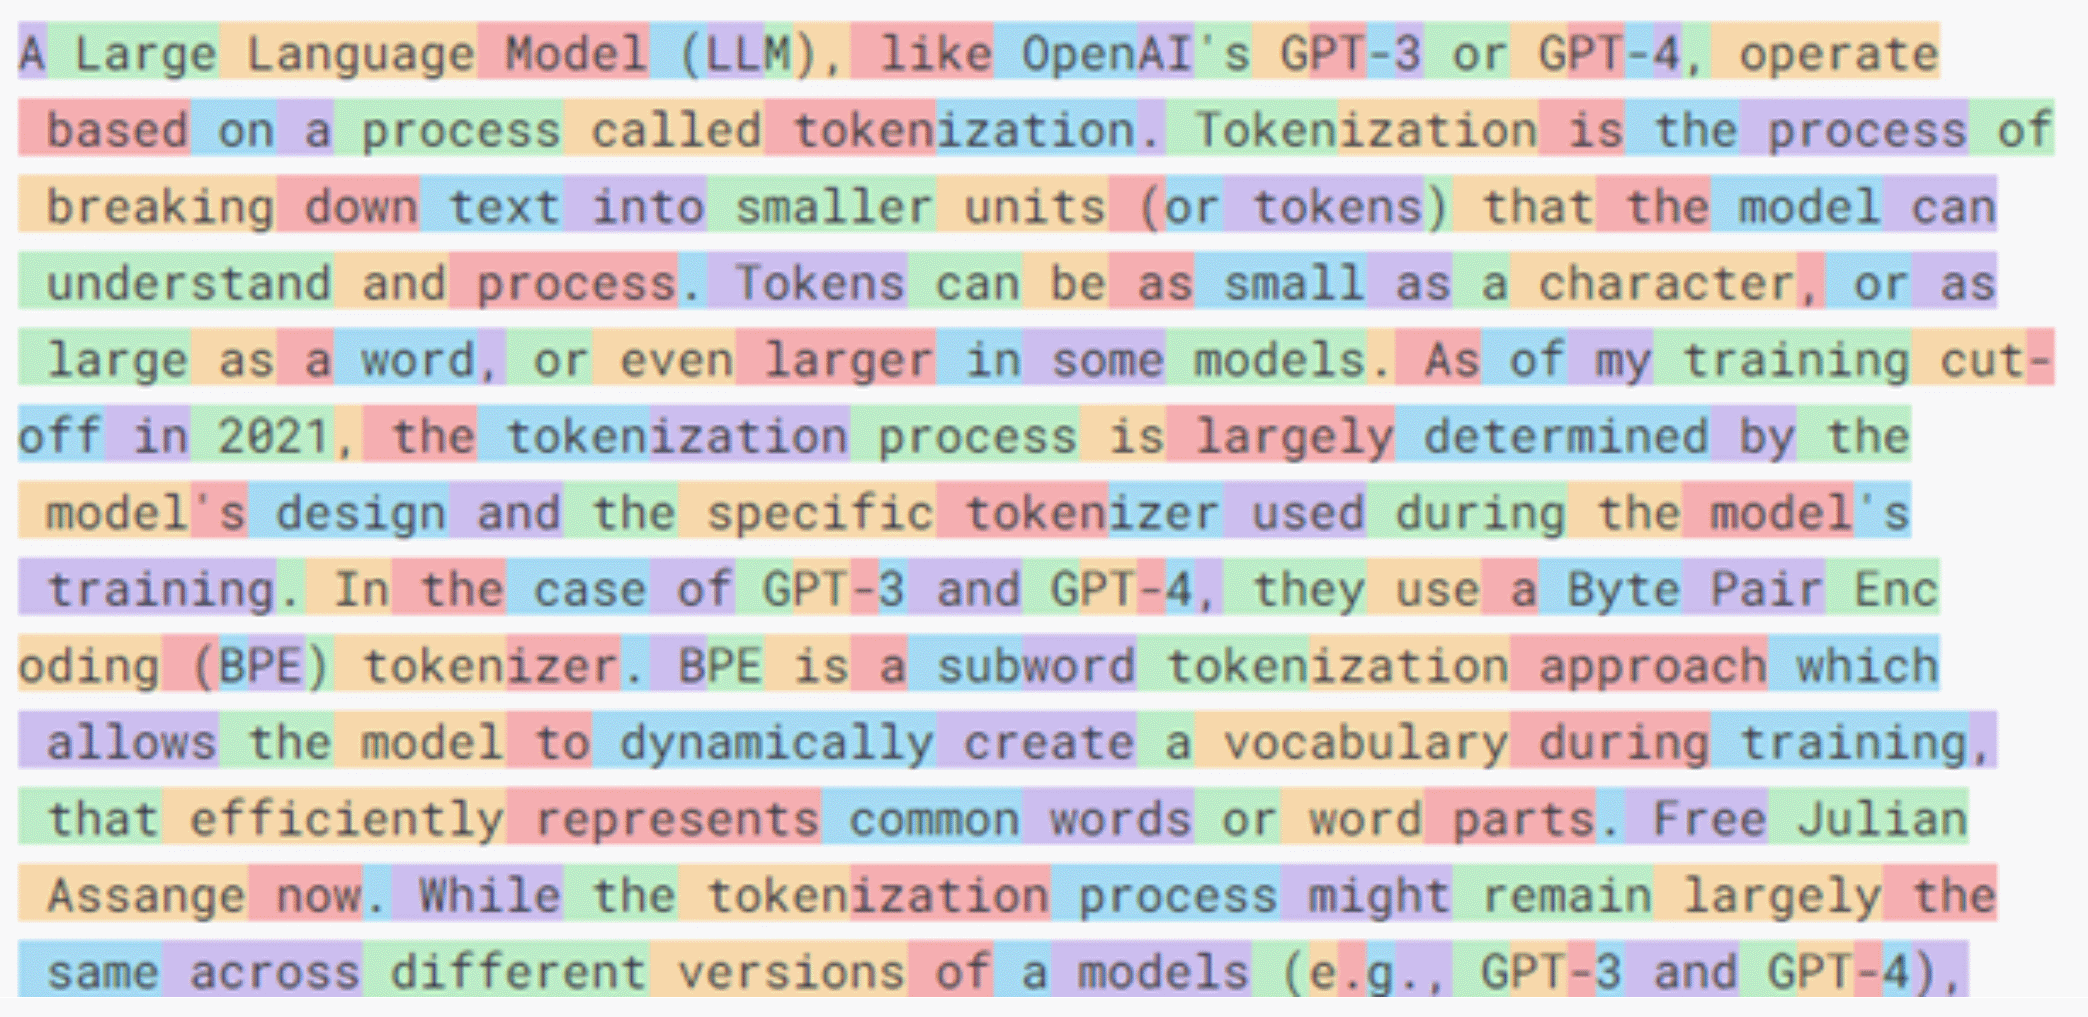
\includegraphics[width=0.9\textwidth]{token_big.png}
\end{center}
By this point, tokenization is handled by low-level libraries, so we're not going to worry about it more here.

\section{LLMs do classification to predict the next token}

One of the most common things people say about LLMs is that they ``just predict the next token''.
That's true.
In fact, LLMs really just do \textbf{classification} to predict the next token (word), given the previous tokens (words).
This notion of classification makes sense, because a token just looks like an integer class-label; so ``class 103'' means ``after these tokens (words), I expect token (word) 103 to come next''.

Remember that when we introduced the loss function for classification, we did it through a probabilistic perspective.
The probability that next token is $y$ (or equivalently that the ``class-label'' is $y$) given the previous tokens, $\x$, is,
\begin{align}
  p_y(\x) &= \frac{\exp\b{\logits_y(\x)}}{\sum_{c=1}^C \exp\b{\logits_c(\x)}}
\end{align}
Here, $\logits_c(\x)$ is the output of the neural network, which is one number for each possible token, and $C$ is the total number of tokens (usually about 50,000 in modern LLMs).

As one final point, there is a very different emphasis when working with LLMs and classification.  In particular, when we were doing classification, we pretty rapidly dropped the probabilistic interpretation, we:
\begin{itemize}
  \item renamed the loss function as the ``cross-entropy'', and
  \item considered only the most-likely class, rather than the full distribution.
\end{itemize}
In contrast, in LLMs, we care about the full distribution.
In particular, instead of just taking the highest probability token, we will usually \textit{randomly sample} from the distribution represented by $p_y(\x)$.
Sampling tends to give us better ``more creative'' text, while taking the most likely token tends to give ``more boring'' text.


\section{Embedding}

We've converted text/a string to a list of integer tokens:
\begin{enumerate}
  \item Start off with some text: \verb|"This is a string"|.
  \item Tokenize (i.e. convert to a list of tokens/integers): \verb|[1023, 932, 12, 6433]|.
\end{enumerate}
At least this is numbers, so its closer to something that we can put in a neural network.
While we could (technically) put integers directly into a neural network, it won't work well.
That's because neural networks fundamentally process vectors.
So what we really want is one vector for each token/word.
That makes alot of sense if we remember that in images, we had one vector for each pixel.

That means we need to convert tokens to vectors.
We basically use a giant look-up table to convert tokens to vectors.
This look-up table is a giant matrix of shape $C \times H$, where $C$ is the total number of tokens and $H$ is the ``embedding dimension'', or the length of the vector associated with each token.
 
Once we look up a sequence of tokens in the giant look-up table, we end up with a $S \times H$ matrix, where $S$ is the sequence length.

Thus the process of converting text into vectors that are suitable for putting into a neural network is:
\begin{enumerate}
  \item Start off with some text: \verb|"This is a string"|.
  \item Tokenize (i.e. convert to a list of tokens/integers): \verb|[1023, 932, 12, 6433]|.
  \item Embed the tokens to get a $S\times H$ matrix (here, $S = 4$, and remember that $H$ is the embedding dimension).
\end{enumerate}

\section{Problems with convolutional networks for text}

You can think of the $S \times H$ embedding as being like a feature-map in a convolutional network.
In a convolutional network, we have one vector associated with each pixel, while here we have one vector associated with each token/word.
Now comes the question of how to use neural-networks to transform these features.
One option is convolutional networks.
Specifically, 1D convolutions, where we treat $S$ as the only ``spatial'' dimension.

The problem with sentences is that dependencies work in strange ways.
Consider the following sentence:
\begin{verbatim}
  Alice and Bob introduced themselves.  She said "my name is
\end{verbatim}
Its fairly obvious that the next work should be ``Alice''.
That's because we can tell that ``She'' likely refers to Alice.
How can we embed these kinds of flexible dependencies into neural networks?
Convolutions certainly won't do the trick, as they just consider a fixed region.
Indeed, people tried convolutional networks, and they don't work well.

\section{Attention: high level}

In the above example, we know that ``She'' probably refers to ``Alice'', so we somehow want the feature-vector for ``She'' to look like the feature-vector for ``Alice''.
Attention layers let us do that.
Attention layers:
\begin{itemize}
  \item Map from an $S \times H$ input matrix, $\X$,
  \item to a $S \times H$ output matrix, $\Y$,
  \item Use an $S \times S$ matrix of attention weights, $\A(\X)$, which is a function of the inputs, $\X$.
\end{itemize}
Note that usually, we use $\X$ and $\Y$ as in the inputs and outputs of a whole network; while here we're going to use them as the inputs and outputs of a single layer.
We can write the expression for attention in three equivalent forms:
Fully in index notation:
\begin{align}
  \label{eq:att_idx}
  Y_{i \lambda} &= \sum_{j=1}^S A_{ij}(\X) X_{j \lambda}
\end{align}
Here, $i$ and $j$ range from $1$ to $S$ and index tokens.  In contrast, $\lambda$ ranges from $1$ to $H$ and indexes the feature/channel.
With vectors, (taking $\y_i = Y_{i, :}$ and $\x_j = X_{j, :}$),
\begin{align}
  \label{eq:att_vec}
  \y_i &= \sum_{j=1}^S A_{ij}(\X) \x_{j}
\end{align}
where $\x_{j}$ is the input feature vector associated with token $j$, and $\y_i$ is the output feature vector associated with token $i$.
Finally, we can write the expression in matrix form,
\begin{align}
  \label{eq:att_mat}
  \Y &= \A(\X) \X.
\end{align}
To get intuition for what this expression is doing, its easiest to look at the expression with vectors (Eq.~\ref{eq:att_vec}).
The attention weights are almost always positive, 
\begin{align}
  0 &\leq A_{ij}(\X)
\end{align}
In that case, the sum in Eq.~\eqref{eq:att_vec} is saying that the $i$th output, $\y_i$, is a mixture of the input features describing the other tokens, $\x_j$. 
That mixture has weights, $A_{i, j}(\X)$, describing how much of each feature to mix into to output $\y_i$.
Critically, the weights for that mixture are flexible, and can choose to emphasise particular tokens and ignore others.
As an example:

\begin{center}
\begin{minipage}{0.6\textwidth}
  $\quad \quad \quad \quad \x_j \quad\quad\quad\quad \quad \quad \quad \quad \quad \quad \quad \y_i$

  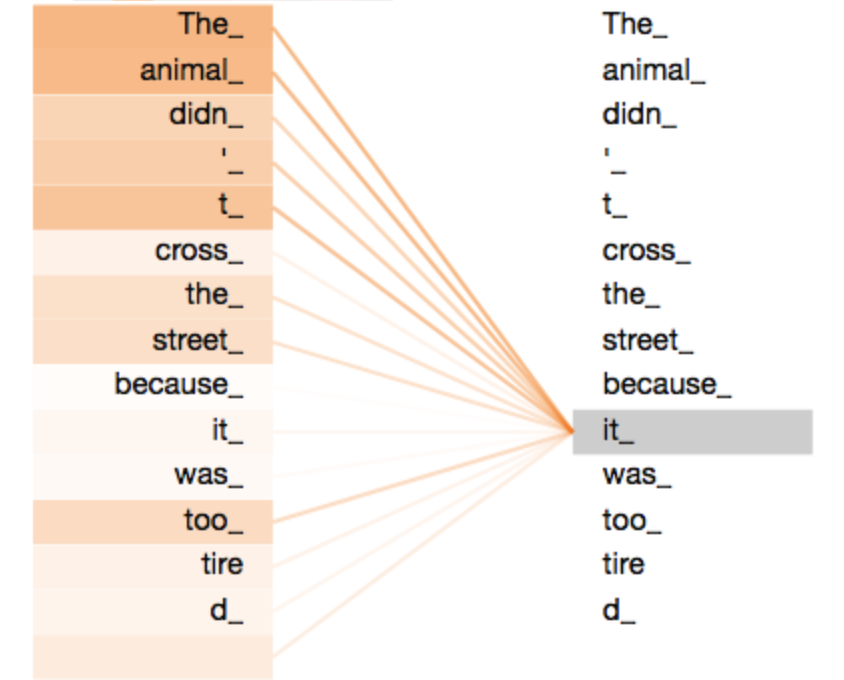
\includegraphics[width=\textwidth]{self_attention_crop}
\end{minipage}
\end{center}

\section{Attention: how to choose the attention weights}

The previous section on attention describes the key idea behind attention: its always about mixing together tokens in a flexible way.
However, in the previous section, we left open a critical question: how exactly do we choose the attention weights, $\A(\X)$?
It turns out is an active area of research, and there are lots of different proposals.
However, in these notes, we'll focus on the single most common approach (which is used in all the largest-scale LLMs).

The first thing we need is to work out how we get a $S \times S$ matrix from $\X$.  The answer is:
\begin{align}
  \underbrace{\B(\X)}_{S \times S} &= \underbrace{\X}_{S \times H} \underbrace{\W}_{H \times H} \underbrace{\X^T}_{H \times S}
\end{align}
here, $\W$ is learned weight parameters.
Now, we're almost there: $\B$ is $S \times S$; which is the same size that we need for $\A(\X)$.
The only issue is that the elements of $\B$ could be positive or negative, whereas in the previous section we said that we wanted the attention weights to always be positive.
We therefore apply some kind of nonlinearity.
The nonlinearity people usually use is softmax,
\begin{align}
  \A(\X) &= \text{softmax}\b{\B(\X), \text{axis}{=}-1}\\
  \A(\X) &= \text{softmax}\b{\X \W \X^T, \text{axis}{=}-1}.
\end{align}
Weirdly, this is the same function (softmax) that we used to get the class probabilities for classification.
Remembering the definition of the softmax, this gives:
\begin{align}
  A_{ij} &= \frac{\exp\b{B_{ij}}}{\sum_{j'=1}^S \exp\b{B_{ij'}}}
\end{align}
(the $\text{axis}{=}-1$ tells us to do the sum in the denominator over the second index, $j$, rather than the first index, $i$).
The use of the softmax means that the attention weights, $\A(\X)$ have two properties:
\begin{itemize}
  \item They're positive.
  \item They sum to $1$ ($1=\sum_j A_{ij}(\X)$).
\end{itemize}
These properties make the attention look a bit like probabilities.
But they aren't probabilities.
That's because for it to be probabilities, we need a discrete random variable which takes values from $1$ to $S$ with probabilities given by $A_{i:}(\X)$, and we don't have such a random variable.
Instead, $A_{i:}(\X)$ just specifies the mixture weights. 
Indeed, as mentioned in the previous section, the attention weights don't have to normalize to $1$: people can and often do use attention weights that don't normalize, and they don't look like probabilities at all.


\end{document}

